\documentclass[english,9pt,aspectraio=169]{beamer}
\usepackage{etex}
\usetheme{uzhneu-en-informal}
%\usepackage{uarial}
\usepackage[T1]{fontenc}
\usepackage[utf8]{inputenc}
\RequirePackage{graphicx,ae}
\usepackage{bm}
\usepackage{fancybox,amssymb,color}
\usepackage{pgfpages}
\usepackage{booktabs}
\usepackage{verbatim}
\usepackage{animate}
\usepackage{numprint}
\usepackage{dsfont}
\usepackage{tikz}
\usepackage{amsmath,natbib}
\usepackage{mathbbol}
\usepackage{babel}
\usepackage{SweaveSlides}
\usepackage{multicol}


\usetheme{uzhneu-en-informal}
\DeclareMathOperator{\po}{Poisson}
\DeclareMathOperator{\G}{Gamma}
\DeclareMathOperator{\Be}{Beta}
\DeclareMathOperator{\logit}{logit}
\def\n{\mathop{\mathcal N}}

\definecolor{Gray}{RGB}{139,137,137}
\definecolor{darkred}{rgb}{0.8,0,0}
\definecolor{Green}{rgb}{0,0.8,0.3}
\definecolor{Blue}{rgb}{0,0,1}
\def\myalert{\textcolor{darkred}}
\def\myref{\textcolor{Gray}}
\setbeamercovered{invisible}

\renewcommand{\baselinestretch}{1.2}
\beamertemplateballitem
\DeclareMathOperator{\cn}{cn} % Copy number
\DeclareMathOperator{\ccn}{ccn} % common copy number
\DeclareMathOperator{\p}{p} % common copy number
\DeclareMathOperator{\E}{E} % common copy number
\DeclareMathOperator{\given}{|} % common copy number
\def\given{\,|\,}
\def\na{\tt{NA}}
\def\nin{\noindent}
\pdfpageattr{/Group <</S /Transparency /I true /CS /DeviceRGB>>}
\def\eps{\varepsilon}

\renewcommand{\P}{\operatorname{\mathsf{Pr}}} % Wahrscheinlichkeitsmaß
\def\eps{\varepsilon}
\def\logit{\text{logit}}
%\newcommand{\E}{\mathsf{E}} % Erwartungswert
\newcommand{\Var}{\text{Var}} % Varianz
\newcommand{\NBin}{\text{NBin}}
\newcommand{\Po}{\text{Po}}


\newcommand{\ball}[1]{\begin{pgfpicture}{-1ex}{-0.65ex}{1ex}{1ex}
\usebeamercolor[fg]{item projected}

{\pgftransformscale{1.75}\pgftext{\normalsize\pgfuseshading{bigsphere}}}
{\pgftransformshift{\pgfpoint{0pt}{0.5pt}}
\pgftext{\usebeamerfont*{item projected}{#1}}}
\end{pgfpicture}}%
\usepackage{multicol}
\newcommand{\ballsmall}[1]{\begin{pgfpicture}{-1ex}{-0.65ex}{.2ex}{.2ex}
\usebeamercolor[fg]{item projected}

{\pgftransformscale{1}\pgftext{\normalsize\pgfuseshading{bigsphere}}}
{\pgftransformshift{\pgfpoint{0pt}{0.5pt}}
\pgftext{\usebeamerfont*{item projected}{#1}}}
\end{pgfpicture}}%


\begin{document}

\frame{
\title[]{ \centering \Huge Kurs Bio144: \\
Datenanalyse in der Biologie}%\\[.3cm]
\author[Stefanie Muff, Owen L.\ Petchey]{\centering Stefanie Muff (Vorlesung) \& Owen L.\ Petchey (Praktikum)}
%\institute[]{Institute of Social and Preventive Medicine \\ Institute of Evolutionary Biology and Environmental Studies}
\date[]{1. Woche: Einf\"uhrung und Ausblick\\ 23./24. Feburar 2017}


\maketitle
}



\frame{\frametitle{Organisatorisches}
Gebe hier genaue Testatbedingungen, Pr\"ufungsdaten (falls bekannt);
OpenEdx Kursseite (Link). Studis m\"ussen sich da anmelden.
}


\frame{\frametitle{Lehrmittel und Literatur}
Obligatorische Lehrmittel:
\begin{enumerate}[1.]
\item \emph{Lineare Regression} von W. Stahel (pdf auf Kurshomepage)
\item \emph{Getting Started With R} von A.P. Beckerman und O.L. Petchey, Oxford University Press;
ISBN 978-0-19-960162-2
\item \emph{The New Statistics With R} von A. Hector, Oxford University Press;
ISBN 978-0-19-872906-8 \\[5mm]
\end{enumerate}

\begin{center}

\includegraphics[width=3cm]{pictures/petchey_buch.jpeg} \qquad \qquad

\includegraphics[width=3cm]{pictures/hector.jpeg}
\end{center}

}

\frame{
\frametitle{Erg\"anzende Literatur:}
\begin{itemize}
\item \emph{Statistics – An Introduction Using R} von M.J. Crawley (\"ahnlich wie 3.) oben)\\[3mm]
\item \emph{The Analysis of Biological Data} von M.C. Whitlock und D. Schluter\\[3mm]
\item \emph{Regression - Modelle, Methoden und Anwendungen} von Fahrmeier, Kneib, Lang
\end{itemize}
}

\frame{\frametitle{Ziele dieses Kurses}
\begin{itemize}
\item Solides Fundement an statistischen Methoden erarbeiten, um biologische oder biomedizinische Fragen mit Daten quantitativ und objektiv zu beantworten.\\[2mm]
\item F\"ahigkeit vermitteln, Resultate in Forschungsartiken zu verstehen, zu interpretiern und evtl. kritisch zu hinterfragen.\\[2mm]
\item Die \emph{Sprache} des Statistikers verstehen lernen.\\[2mm]
\item Wir m\"ochten Euch eine herausforderne, spannende und freudvolle Lernerfahrung geben. {\bf Etwas, was man wirklich brauchen kann und darum Spass macht.}\\[6mm]
\end{itemize}

Meine \"Uberzeugung: Fundierte Kenntnisse in Statistik machen Sie unabh\"angig! \\[2mm]

}

\frame{\frametitle{Voraussetzungen f\"ur Bio144}
\begin{itemize}
\item Mat183 Stochastik f\"ur die Naturwissenschaften
\end{itemize}

}



\frame{\frametitle{Kurs-Fahrplan (12 Wochen)}
\vspace{-8mm}

\begin{multicols}{2}
1. Einf\"uhrung und Ausblick \\[1mm]
2. Einfache lineare Regression\\[1mm]
3. Residuenanalyse, Modellvalidierung \\[1mm]
4. Multiple lineare Regression \\[1mm]
5. ANOVA und ANCOVA \\[1mm]
6. Matrix Algebra \\[1mm]
7. Modellwahl  \\[1mm]
8. Interpretation von Resultaten \\[1mm]
9. Bin\"are Daten (logistische Regression)\\[1mm]
10. Z\"ahldaten (Poisson Regression) \\[1mm]
11. Messfehler, zuf\"allige Effekte \\[1mm]
12. Ausgew\"ahlte Themen, Wiederholungen und Ausblick \\
\end{multicols}
~\\
{\bf Kurzfristige Anpassungen vorbehalten!}
}

\frame{\frametitle{Warum ist Statistik f\"ur die Biologie und Medizin so wichtig?}

Was denken Sie? \\[4mm]



\pause


Erkenntnis, dass ohne Kenntnisse in statistischer Datenanalyse eigene Daten in Bachelor-, Master- oder Doktorarbeiten nicht ausgewertet werden k\"onnen. \\[2mm]

Beispiele:
\begin{itemize}
\item Medizin: Hat ein bestimmtes Medikament eine Wirkung? Welche Faktoren führen zu Krebs?
\item Oekologie: Was für einen Lebensraum braucht ein Tier zum Leben? Was bevorzugt es?
\item Evolutionsbiologie: Haben Tiere mit hohem Inzuchtgrad schlechtere Chancen zu \"uberleben oder sich fortzupflanzen?
\end{itemize}
}

\frame{
Achtung! "Learning by doing" ist in der Statistik praktisch unm\"oglich. Es braucht viel Erfahrung, es gibt sehr viele Fallstricke.\\[5mm]

Wer ein gutes Grundlagenwissen in Statistik hat, kann unabh\"angiger arbeiten. Wer sich nicht auskennt, ist immer auf die Hilfe anderer Leute angewiesen...\\[5mm]

Datenanalyse ist selber ein spannender Teil der Forschung! \\[5mm]
 
Datenanalyse ist die Schnittstelle zwischen Mathematik und Biologie (oder anderen Forschungsfeldern, z.B. Medizin, Geographie etc.).
}


\frame{\frametitle{Was leistet die Datenanalyse?}
\begin{itemize}
\item Auffinden und Quantifizierung von Zusammenh\"angen durch graphische Darstellung und Modellierung.\\[3mm]
\item Aus Daten g\"ultige Schlussfolgerungen ziehen.\\[3mm]
\item Die Unsicherheit der Schlussfolgerung quantifizieren.
\end{itemize}
}

\frame{\frametitle{Eigene Beispiele}
\myalert{\large Fischotter} \citep{weinberger.etal2016}\\[2mm]

\emph{Forschungsfrage:} Welche Lebensr\"aume werden von den Fischottern bevorzug? \\[1mm]
\emph{Methode:} Studie in \"Osterreich, 9 Otter mit Radiotelemetriesendern versehen und w\"ahrend 2-3 Jahren \"uberwacht.\\

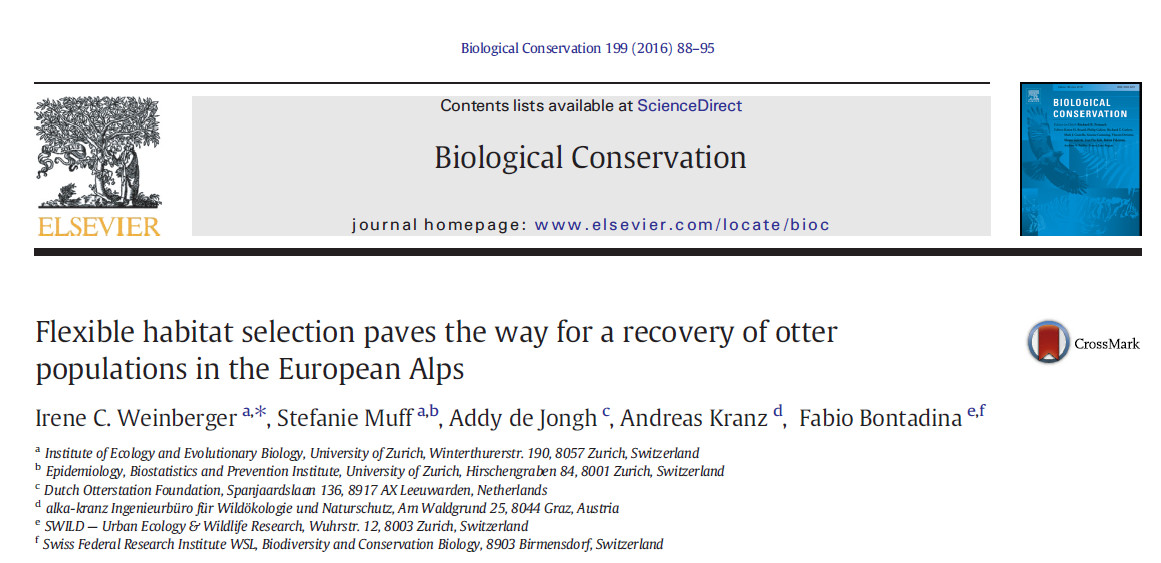
\includegraphics[width=10cm]{pictures/otters.jpeg}
}


\frame{
\myalert{\large Inzucht bei Steinb\"ocken}\\[2mm]

\emph{Forschungsfrage:} Hat Inzucht in Steinbockpopulationen eine negative Auswirkung auf das Langzeit-Populationswachstum? Inzuchtdepression!\\[4mm]

\begin{multicols}{2}
\emph{Methoden:} Genetische Information aus Blutproben gibt Aufschluss \"uber Inzucht der Steinb\"ocke. Langzeit-Monitoring von Populationsgr\"ossen und Abschussquoten.\\[3mm]

%\begin{center}
%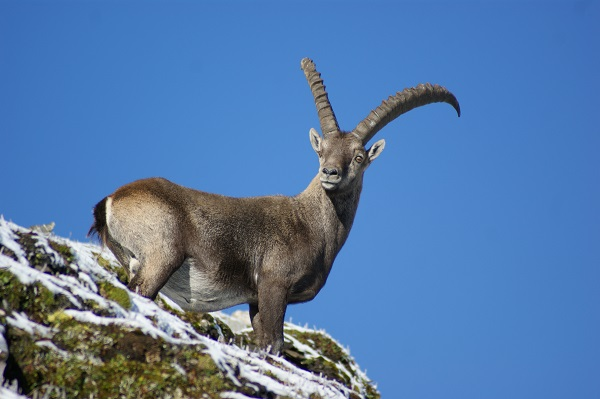
\includegraphics[width=4cm]{pictures/steinbock.jpg} \hspace{1cm}
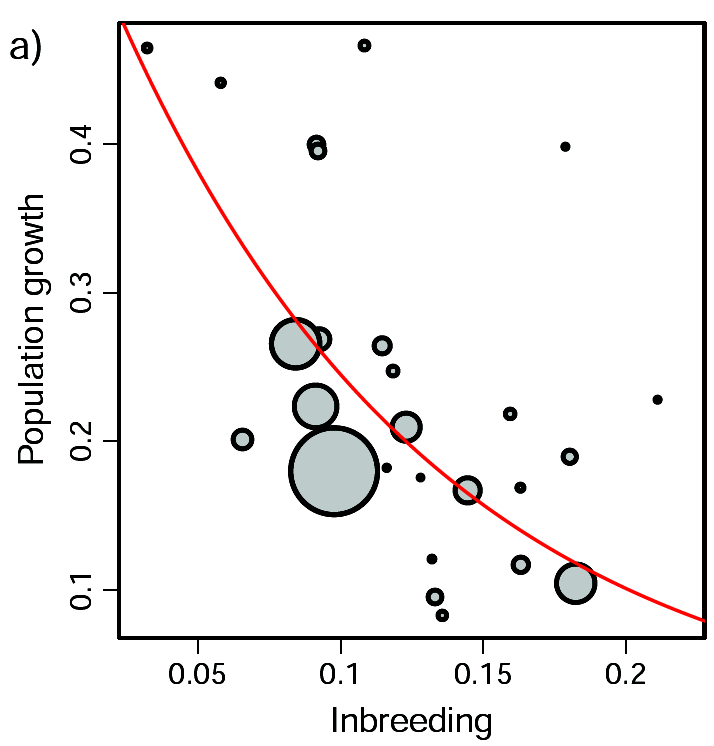
\includegraphics[width=4cm]{pictures/ibex_graph.png}
%\end{center}
\end{multicols}
\vspace{-1cm}
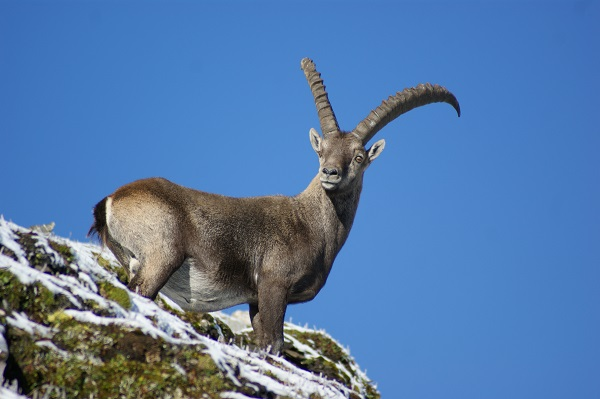
\includegraphics[width=3cm]{pictures/steinbock.jpg}
}

\frame{\frametitle{}
\myalert{Quecksilberbelastung im Boden} \\[2mm]

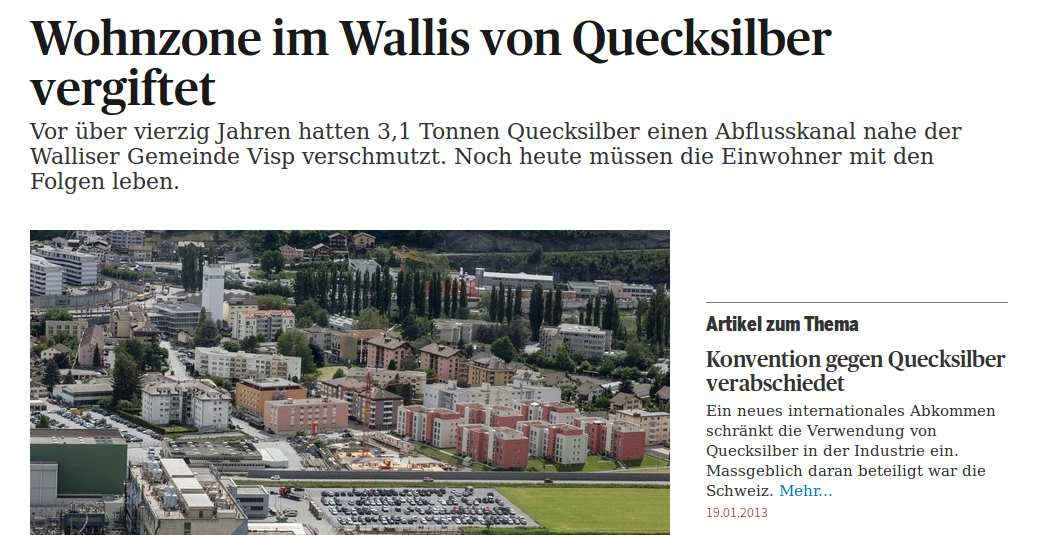
\includegraphics[width=8cm]{pictures/wallis.png} \\[2mm]

\emph{Forschungsfrage:} Gibt es einen Zusammenhang zwischen Quecksilber(Hg)-Bodenwerten von Wohnh\"ausern und der Hg-Belastung im K\"orper (Urin, Haar) der Bewohner? \\[2mm]
\emph{Methode:} Bodenmessungen auf den Grundst\"ucken, sowie Messungen und Befragungen von Kindern und deren M\"uttern.\\[2mm]

Hoch brisante, politisch aufgeladene Fragestellung!\\
\href{http://www.srf.ch/news/regional/bern-freiburg-wallis/quecksilber-im-walliser-boden-schadete-der-gesundheit-nicht}
{\beamergotobutton{Schweiz Aktuell, 20. Juni 2016}}
 
}


\frame{\frametitle{}
\myalert{Bewegungsverhalten bei Kindern} \\[6mm]

%\includegraphics{pictures/g}

\emph{Forschungsfrage:} Welche Einflussfaktoren beeinflussen das Bewegungsverhalten von 3-5 j\"ahrigen Kindern?\\[4mm]

\emph{Methode:} Die Kinder werden w\"ahrend mehreren Tagen mit Bewegungsmessern ausgestattet. Die Eltern m\"ussen mehrmals einen detaillierten Fragebogen ausf\"ullen.\\[4mm]
Erfasste Variablen sind z.B. Medienkonsum, Verhalten der Eltern, Gewicht, Alter,...\\[7mm]

\href{http://splashy.ch/}
{\beamergotobutton{Link zur Splashy Studie}}
 
}



\frame{\frametitle{Statistik in der NZZ (April 2016)}
 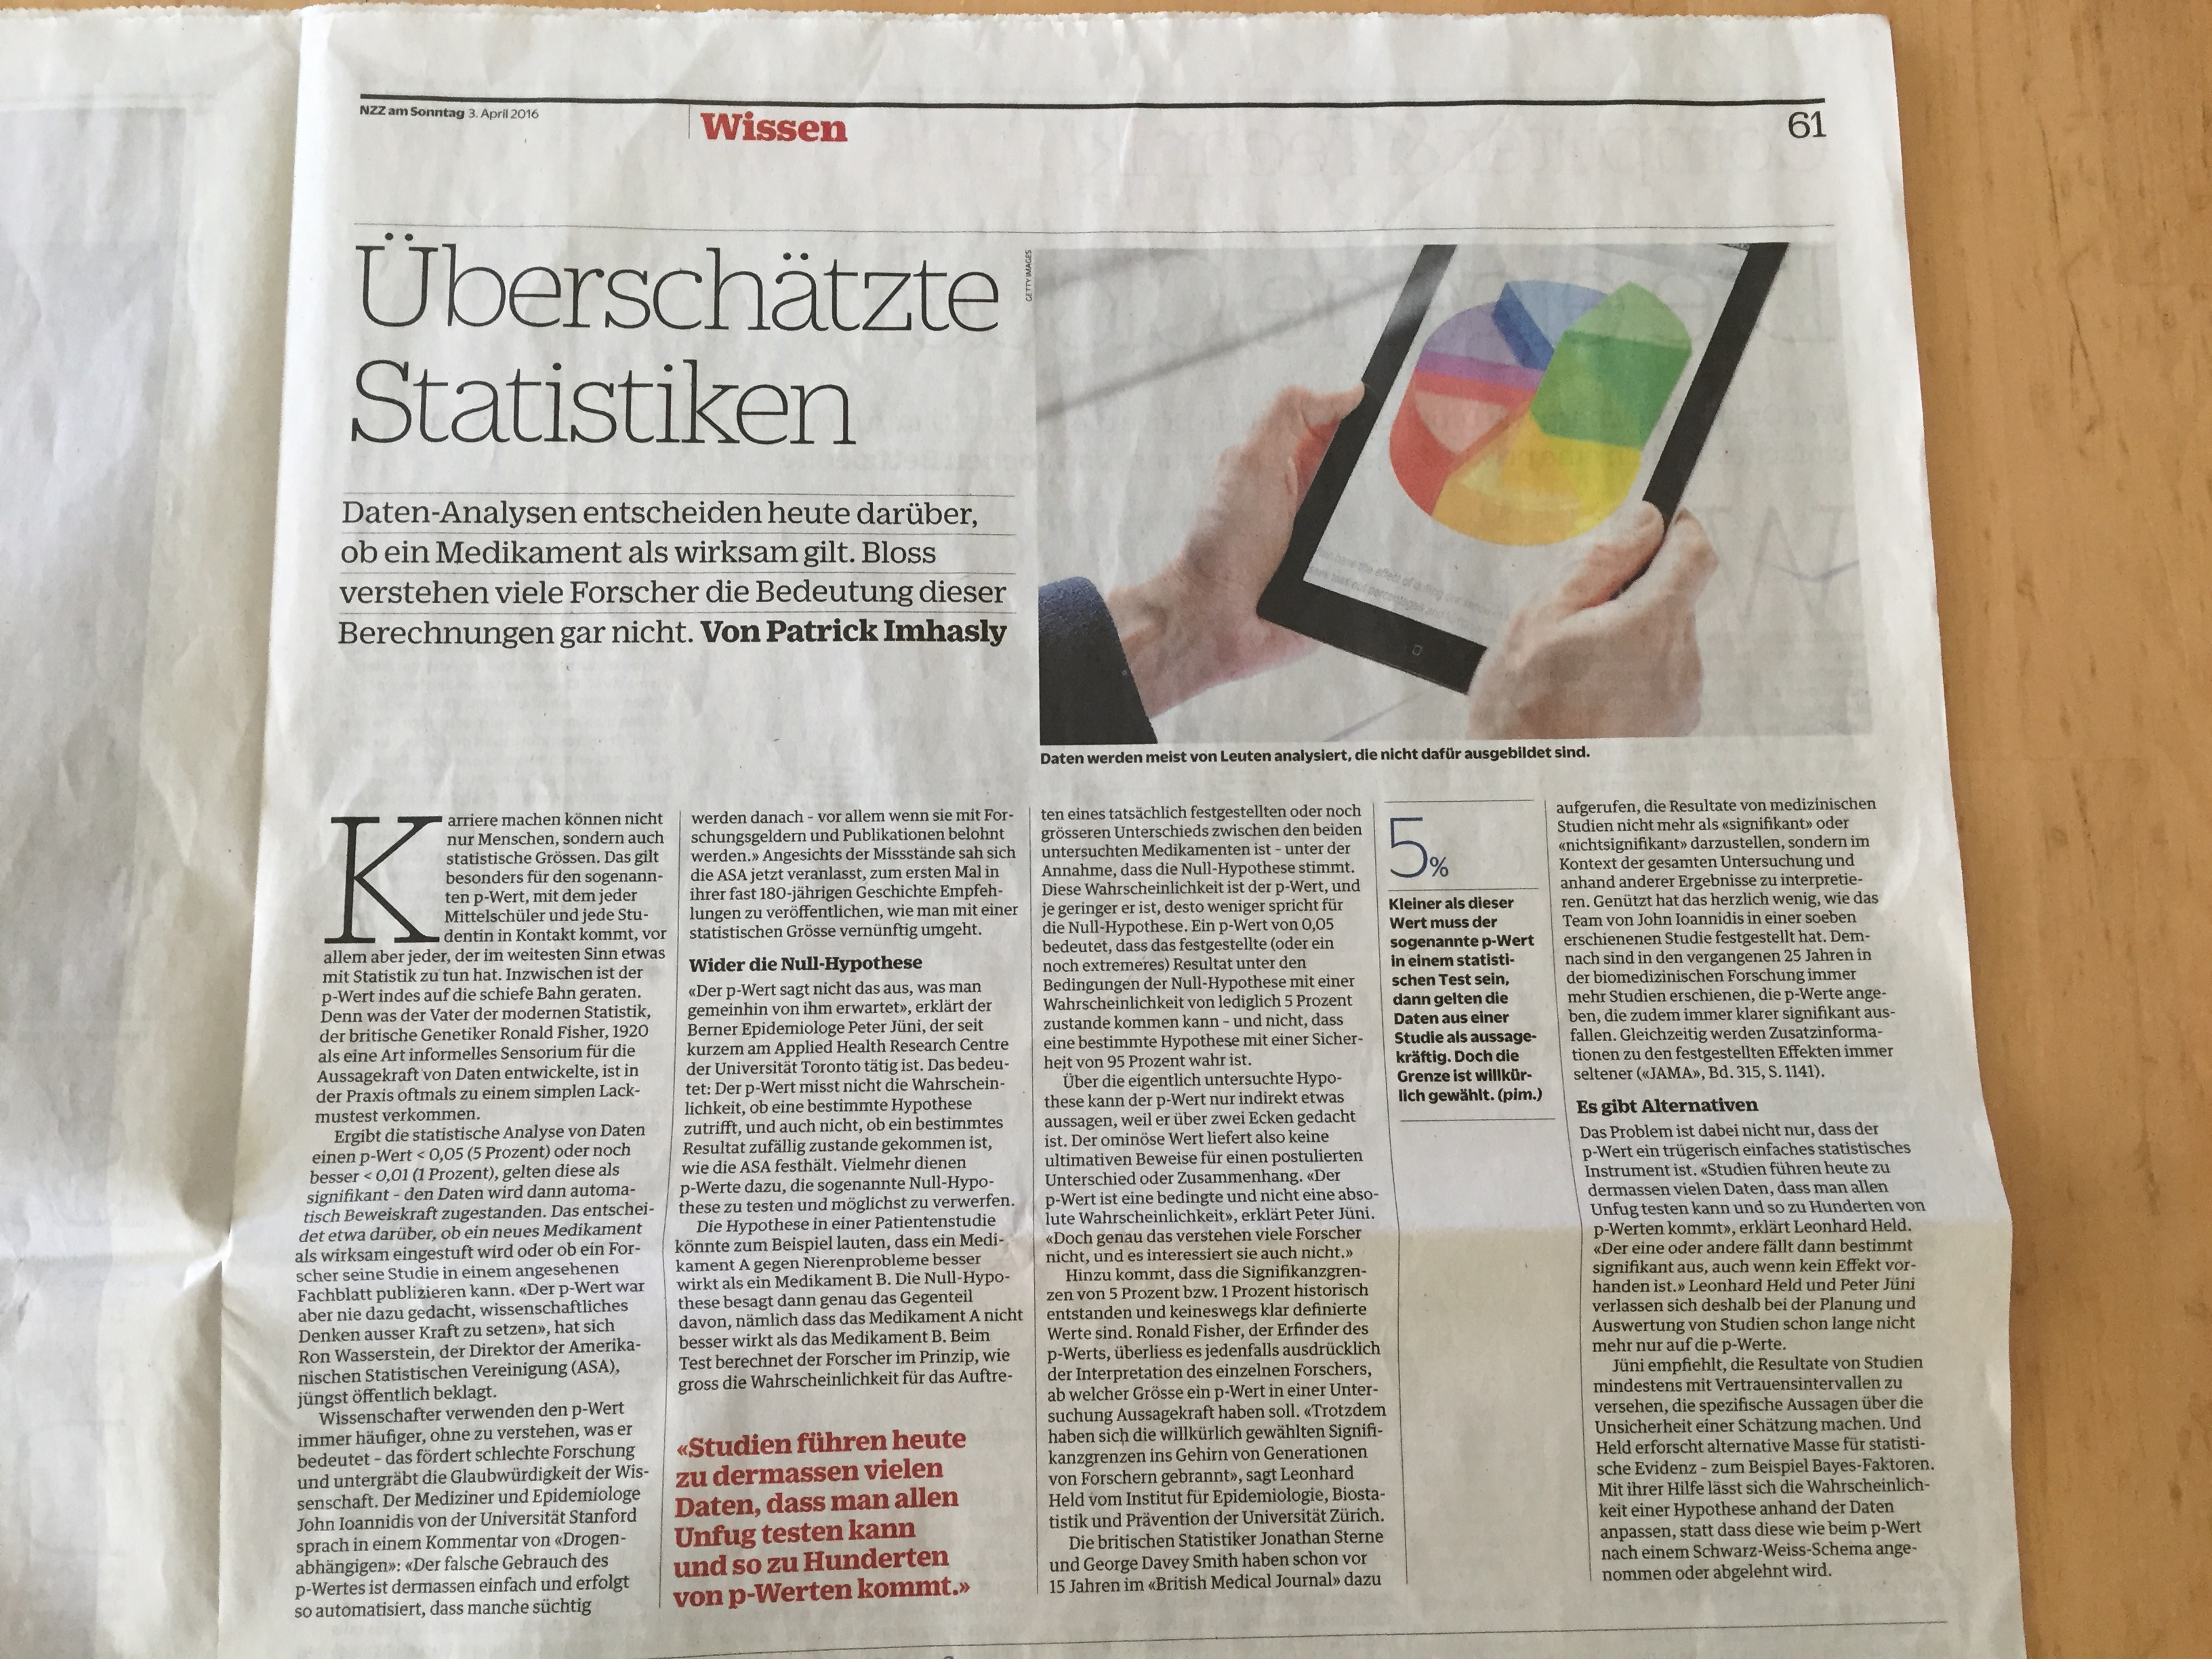
\includegraphics[width=10cm]{pictures/NZZ1.jpeg}
}


\frame[containsverbatim]{\frametitle{Beispiel 1: Prognostische Faktoren f\"ur K\"orperfett}
\vspace{-1cm}
{\scriptsize (Aus Theo Gasser \& Burkhardt Seifert \emph{Grundbegriffe der Biostatistik})}\\[6mm]

K\"orperfett ist ein wichtiger Indikator f\"ur \"Ubergewicht, aber schwer zu messen. \\
{\bf Frage:} welche Faktoren erlauben eine gute Sch\"atzung des K\"orperfetts? \\[4mm]

Studie mit 241 M\"annern, von welchen der K\"orperfett-Anteil (in \%) und andere Variablen wie Alter, Gewicht, K\"orpergr\"osse, BMI, Nackenfett und Bauchumfang gemessen wurden.\\[4mm]

\begin{Schunk}
\begin{Sinput}
> str(d.bodyfat)
\end{Sinput}
\begin{Soutput}
'data.frame':	243 obs. of  7 variables:
 $ bodyfat: num  12.3 6.1 25.3 10.4 28.7 20.9 19.2 12.4 4.1 11.7 ...
 $ age    : int  23 22 22 26 24 24 26 25 25 23 ...
 $ gewicht: num  70 78.7 69.9 83.9 83.7 ...
 $ hoehe  : num  172 184 168 184 181 ...
 $ bmi    : num  23.6 23.4 24.7 24.9 25.5 ...
 $ neck   : num  36.2 38.5 34 37.4 34.4 39 36.4 37.8 38.1 42.1 ...
 $ abdomen: num  85.2 83 87.9 86.4 100 94.4 90.7 88.5 82.5 88.6 ...
\end{Soutput}
\end{Schunk}
 

}


\frame[containsverbatim]{\frametitle{}
 
\setkeys{Gin}{width=0.75\textwidth}
\begin{Schunk}
\begin{Sinput}
> pairs(d.bodyfat)
\end{Sinput}
\end{Schunk}
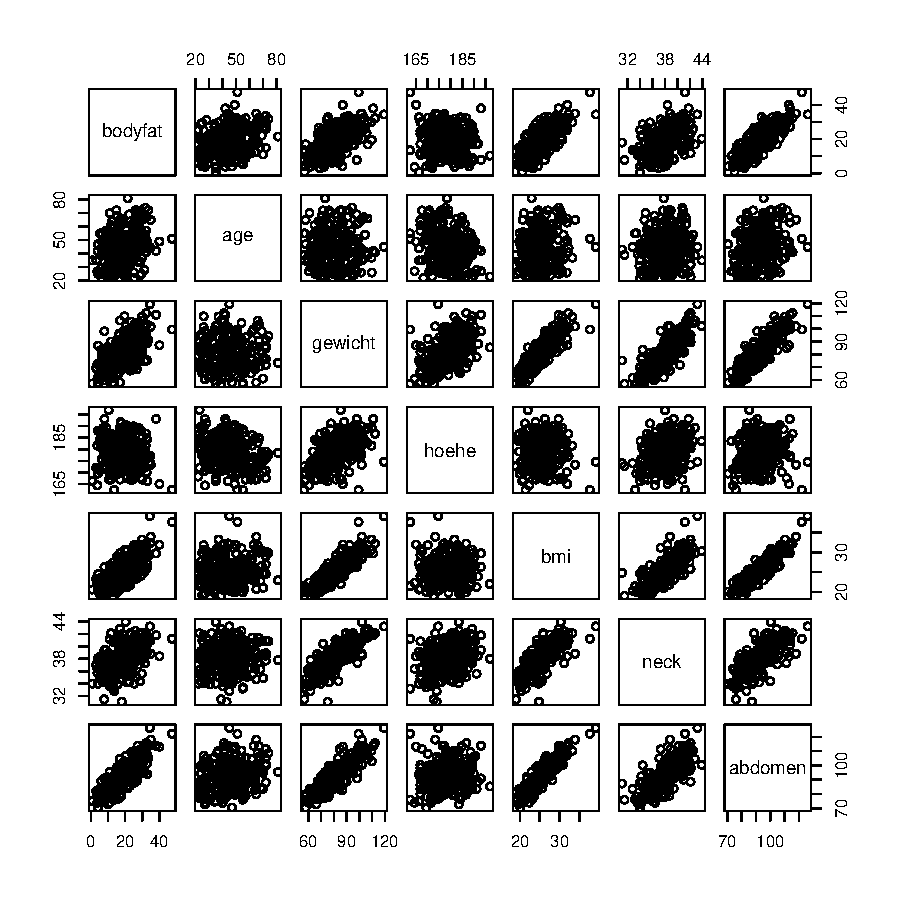
\includegraphics{Bio144_2017_week1-pairs}

\texttt{pairs()} liefert die Streudiagramme (scatterplots) von allen Variablen gegen alle.
}



\frame{\frametitle{}
\vspace{-0.5cm}
\begin{center}
\setkeys{Gin}{width=0.7\textwidth}
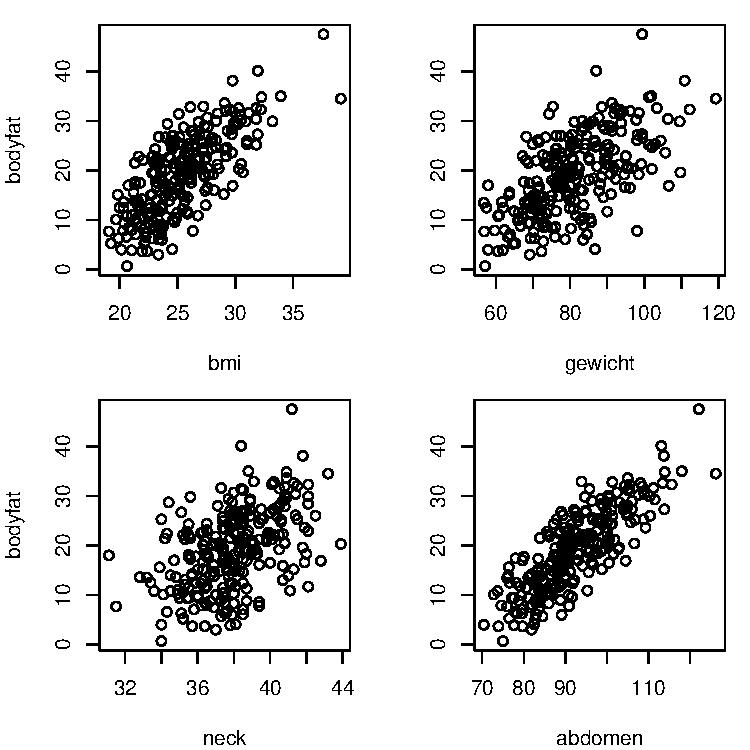
\includegraphics{Bio144_2017_week1-004}
\end{center}

Gesucht ist ein \emph{Modell}, welches das K\"orperfett aus einfach zu messenden Gr\"ossen m\"oglichst genau \myalert{vorhersagen} kann.
}



\frame[containsverbatim]{\frametitle{Beispiel 2: Quecksilber im Wallis}
{\bf Frage:} Zusammenhang zwischen Hg-Werten im Boden und Werten im Urin? Wir verwenden hier ein leicht modifiziertes Datenset.\\[5mm]

\begin{Schunk}
\begin{Sinput}
> str(d.hg)
\end{Sinput}
\begin{Soutput}
'data.frame':	156 obs. of  10 variables:
 $ Hg_urin        : num  0.258 0.036 0.16 0.314 0.29 ...
 $ Hg_soil        : num  0.49 0.42 0.18 0.49 0.24 0.2 0.1 14 0.1 0.3 ...
 $ veg_garden     : int  1 1 1 1 1 1 1 1 1 1 ...
 $ migration      : int  0 0 0 0 0 1 1 0 0 0 ...
 $ smoking        : int  0 0 0 0 0 0 0 0 0 0 ...
 $ amalgam_quant  : int  3 0 2 0 0 0 0 1 0 0 ...
 $ age            : int  51 11 34 8 6 40 7 48 11 38 ...
 $ Meerfisch_quant: int  3 2 5 4 4 2 2 4 0 7 ...
 $ last_time_fish : int  0 0 0 0 0 0 0 0 0 0 ...
 $ mother         : Factor w/ 2 levels "0","1": 2 1 2 1 1 2 1 2 1 2 ...
\end{Soutput}
\end{Schunk}

}


\frame[containsverbatim]{\frametitle{}
\vspace{1cm}
Erste visuelle Inspektion ist nicht sehr informativ. Es ist kein Zusammenhang von Auge ersichtlich:
%
\begin{center}
\setkeys{Gin}{width=0.65\textwidth}
\begin{Schunk}
\begin{Sinput}
> plot(Hg_urin ~ Hg_soil, data=d.hg, xlab="Hg Boden", ylab = "Hg Urin")
\end{Sinput}
\end{Schunk}
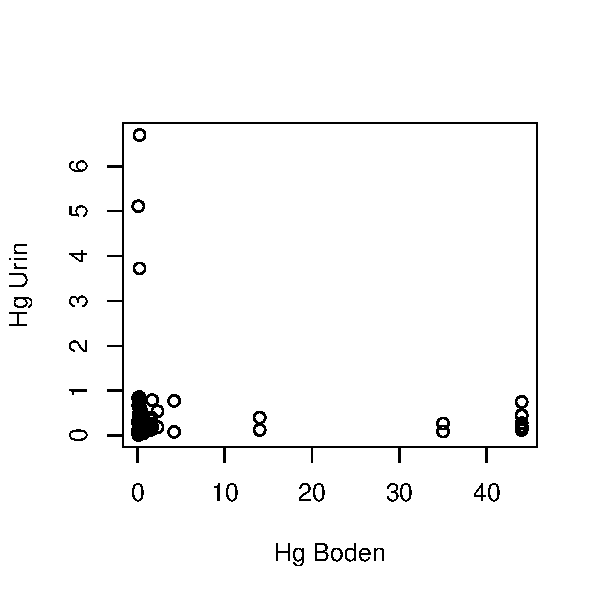
\includegraphics{Bio144_2017_week1-hg1}
\end{center}

}

\frame[containsverbatim]{\frametitle{}
Haben andere Faktoren einen Einfluss auf Hg im Urin?\\[4mm]

\begin{center}
\setkeys{Gin}{width=1.0\textwidth}
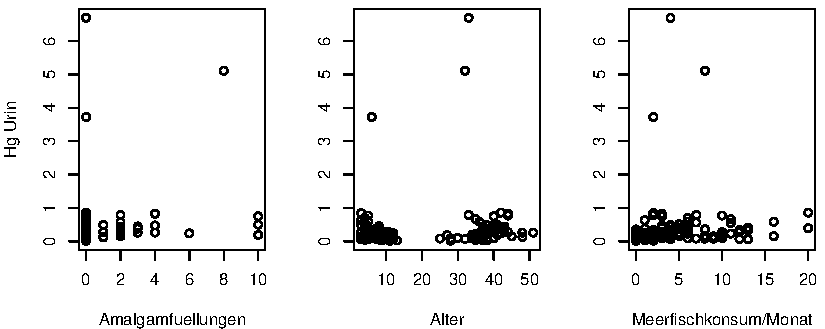
\includegraphics{Bio144_2017_week1-hg2}
\end{center}
\vspace{5mm}

Aus diesen Grafiken is es sehr schwer zu sagen, welche Faktoren die Quecksilberbelastung im Menschen genau beeinflussen.

}


\frame[containsverbatim]{\frametitle{}
Es ist immer n\"utzlich, die Verteilungen der Variablen im Modell anzuschauen. Zeichnen wir mal das Histogramm der Quecksilberwerte:\\[4mm]

\begin{center}
\setkeys{Gin}{width=0.9\textwidth}
\begin{Schunk}
\begin{Sinput}
> par(mfrow=c(1,2))
> hist(d.hg$Hg_soil,xlab="Hg Boden",nclass=20,main="")
> hist(d.hg$Hg_urin,xlab="Hg Urin",nclass=20,main="")
\end{Sinput}
\end{Schunk}
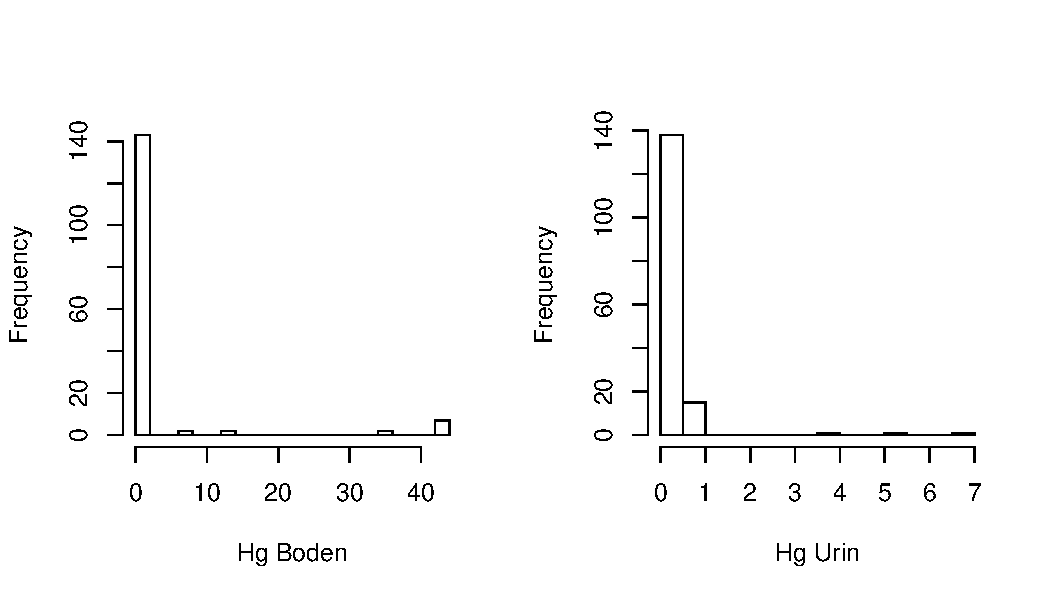
\includegraphics{Bio144_2017_week1-hghist}
\end{center}

Es zeigt sich: fast alle Hg-Werte ``kleben'' bei 0.

}

\frame[containsverbatim]{\frametitle{}
In solchen F\"allen kann es helfen, die Variable zu \emph{logarithmieren}.

 \begin{center}
\setkeys{Gin}{width=0.9\textwidth}
\begin{Schunk}
\begin{Sinput}
> par(mfrow=c(1,2))
> hist(log(d.hg$Hg_soil),xlab="log(Hg Boden)",nclass=20,main="")
> hist(log(d.hg$Hg_urin),xlab="log(Hg Boden)",nclass=20,main="")
\end{Sinput}
\end{Schunk}
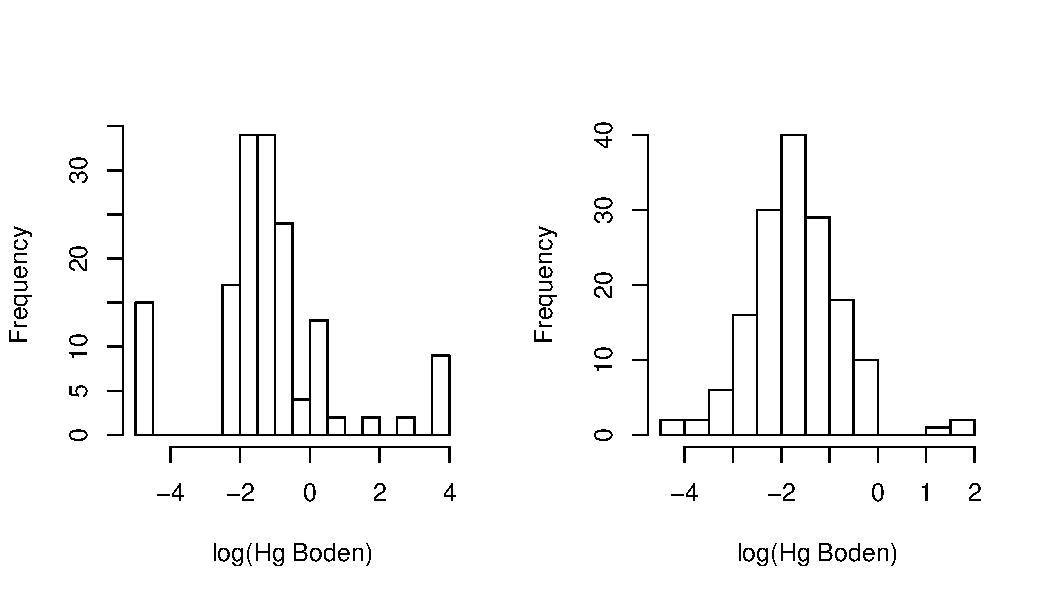
\includegraphics{Bio144_2017_week1-hghist2}
\end{center}
}

\frame[containsverbatim]{\frametitle{}
Mit logarithmierten Werten sieht auch das Streudiagramm etwas sinnvoller aus:

\begin{center}
\setkeys{Gin}{width=0.5\textwidth}
\begin{Schunk}
\begin{Sinput}
> plot(log(Hg_urin) ~ log(Hg_soil), data=d.hg, xlab="Hg Boden", 
+      ylab = "Hg Urin",pch=21,bg=as.numeric(mother)+2,xlim=c(-4.5,4.5))
> legend("topright",legend=c("Kinder","Muetter"),col=c(3,4),pch=21,pt.bg=c(3,4))
\end{Sinput}
\end{Schunk}
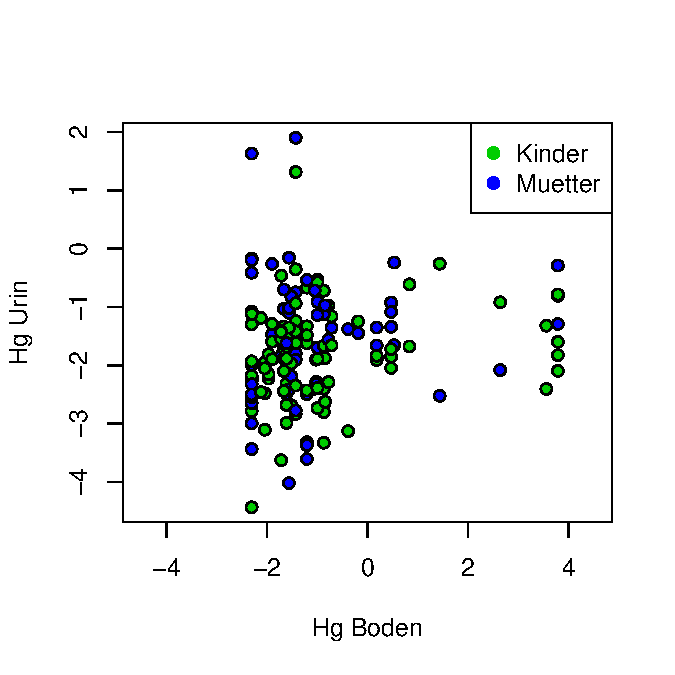
\includegraphics{Bio144_2017_week1-hg1_log}
\end{center}

Merke: Auf die Idee, die Variablen zu logarithmieren, sind wir nur dank visueller Inspektion gekommen.
}





\frame[containsverbatim]{\frametitle{Beispiel 3: Ern\"ahrung und Blutzucker}
\vspace{-3mm}
{\scriptsize\citep[p. 190]{elpelt.hartung1987}}\\[2mm]
%
24 Personen werden in 4 Gruppen unterteilt. Jede Gruppe erh\"alt eine andere Di\"at \small{(DIAET)}. Es werden zu Beginn und am Ende (nach 2 Wochen) die Blutzuckerwerte gemessen. Die Differenz wird gespeichert \small{(BLUTZUCK)}.\\[2mm]
{\bf Frage:} Unterscheiden sich die Gruppen in der Ver\"anderung der Blutzuckerwerte?\\[3mm]

\begin{center}
\setkeys{Gin}{width=0.7\textwidth}
\begin{Schunk}
\begin{Sinput}
> par(mfrow=c(1,2))
> plot(BLUTZUCK ~ DIAET,d.blz,xaxt="n",main="Streudiagramm")
> axis(1,1:4)
> boxplot(BLUTZUCK ~ DIAET,d.blz,xaxt="n",xlab="DIAET",main="Boxplot")
> axis(1,1:4)
\end{Sinput}
\end{Schunk}
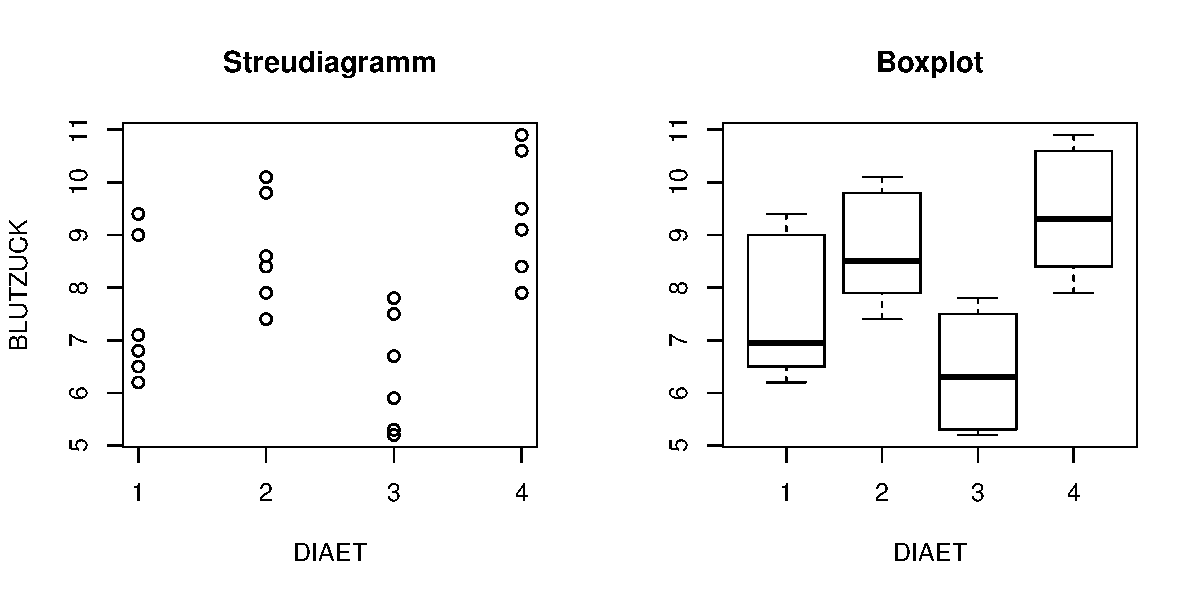
\includegraphics{Bio144_2017_week1-blz_plot}
\end{center}

}


\frame[containsverbatim]{\frametitle{}
Kommt Ihnen diese Fragestellung irgendwie bekannt vor? \\
Stichwort: 2 Gruppen. \\[4mm]

F\"ur mehrere Gruppen braucht man die \emph{Varianzanalyse} oder \emph{ANOVA} (=ANalysis Of VAriance).\\[4mm]

Es wird sich herausstellen (Woche 5), dass sich die Di\"aten tats\"achlich voneinander unterscheiden. \\[4mm]

Die n\"achste Frage ist dann, welche Di\"aten sich \emph{paarweise} voneinander unterscheiden.
}

\frame[containsverbatim]{\frametitle{Beispiel 4: Blut-Screening}
\vspace{-5mm}
{\scriptsize\citep[Aus ][Chapter 7.1]{hothorn.everitt2014}}\\[4mm]

Untersucht wird, ob eine hohe ESR (erythrocyte sedimentation rate) ein Indikator f\"ur gewisse Krankheiten (Rheuma, chronische Entz\"undungen etc) ist.\\[3mm]

{\bf  Konkret: } Gibt es einen Zusammenhang zwischen einem ESR Level ESR$<20mm/hr$ und den Plasmaproteinen Fibrinogen und Globulin?\\[3mm]

Lade die Daten aus dem Package, welches f\"ur \citet{hothorn.everitt2014} geschrieben wurde:\\[2mm]

\begin{Schunk}
\begin{Sinput}
> library(HSAUR3)
> data("plasma",package="HSAUR3")
\end{Sinput}
\end{Schunk}
\begin{Schunk}
\begin{Sinput}
> plasma[c(1,5,9,10,15,29),]
\end{Sinput}
\begin{Soutput}
   fibrinogen globulin      ESR
1        2.52       38 ESR < 20
5        3.41       37 ESR < 20
9        3.15       39 ESR < 20
10       2.60       41 ESR < 20
19       2.60       38 ESR < 20
15       2.38       37 ESR > 20
\end{Soutput}
\end{Schunk}
}

\frame[containsverbatim]{\frametitle{}
Die Unterteilung ESR$<20mm/hr$ vs.\ ESR$\geq 20mm/hr$ f\"uhrt zu einer \myalert{bin\"aren} Variable.\\

Der Zusammenhang der einzelnen Plasmaprotein-Levels kann mit einer grafischen Darstellung, dem \emph{conditional density plot}, gut erfasst werden:

\begin{center}
\setkeys{Gin}{width=0.9\textwidth}
\begin{Schunk}
\begin{Sinput}
> par(mfrow=c(1,2))
> cdplot(ESR ~ fibrinogen,plasma)
> cdplot(ESR ~ globulin,plasma)
\end{Sinput}
\end{Schunk}
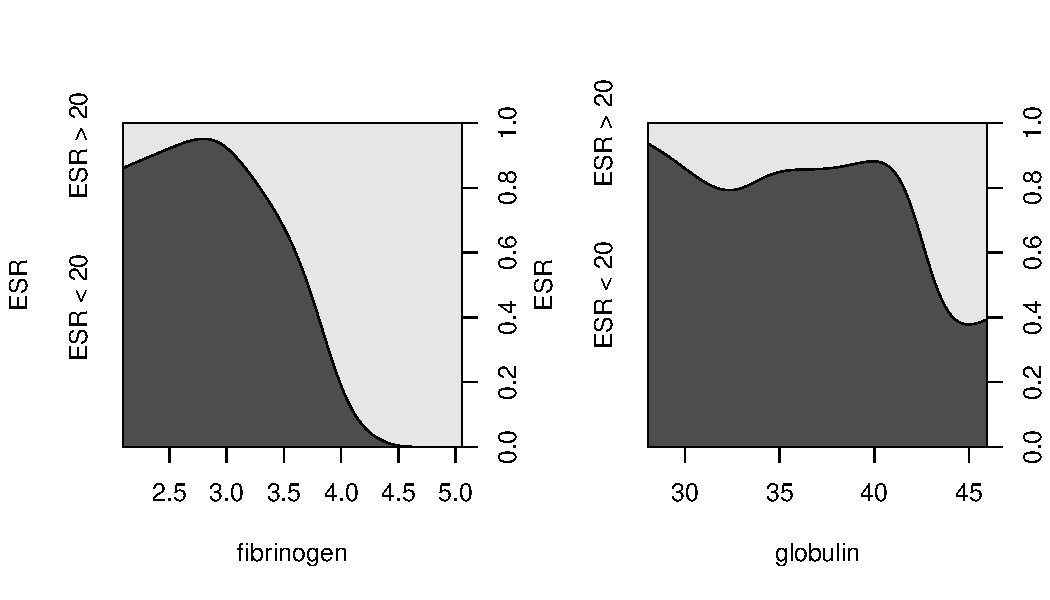
\includegraphics{Bio144_2017_week1-cdplot_ESR}
\end{center}

}


\frame{\frametitle{Was ist ein Modell?}
Ein Modell ist eine Ann\"aherung an die Realit\"at. Das Ziel der Statistik und Datenanalyse ist es immer, dank Vereinfachungen der wahren Welt gewisse Zusammenh\"ange zu erkennen.\\[6mm]

David Hand schrieb 2014:\\[4mm]

\emph{In general, when building statistical models, we must
not forget that the aim is to understand something about
the real world. Or predict, choose an action, make
a decision, summarize evidence, and so on, but always
about the real world, not an abstract mathematical
world: our models are not the reality -- a point well
made by George Box in his oft-cited remark that \myalert{``all
models are wrong, but some are useful'' \citep{box1979}.}
}

}


\frame{\frametitle{Vorgehen bei einem Modellierungsprozess}
\begin{enumerate}
\item Pr\"azise Fragestellung formulieren
\item Datenerhebung und -analyse planen, Daten sammeln (Experimente, Erhebungen)
\item Daten aufbereiten und bereinigen
\item Daten graphisch darstellen
\item Ein geeignetes \emph{Modell} ausw\"ahlen
\item Modellparameter und deren Unsicherheit sch\"atzen
\item Modellannahmen \"uberpr\"ufen
\item Falls notwendig, Modell verbessern; zur\"uck zu Schritt 7
\item Resultate interpretieren und mit Schritt 1 vergleichen
\item Resultate pr\"azise und verst\"andlich kommunizieren (Publikation, Zeitungsbericht...)
\end{enumerate}

}


\frame{\frametitle{Fragestellungen der Datenanalyse}
\begin{enumerate}[a)]
\item \myalert{Vorhersage, Interpolation}. Beispiel K\"orperfett: verwende Ersatzumessungen, um K\"orperfett einer Person vorherzusagen.\\[3mm]
\item \myalert{Sch\"atzung von Parametern} (Beispiel: ...)\\[3mm]
\item \myalert{Bestimmung von Einflussgr\"ossen}. Beispiel Aktivit\"atsstudie bei Kindern: Es werden Faktoren gesucht, welche das Bewegungsverhalten der Kinder (positiv oder negativ) beeinflussen.\\[3mm]
\item Optimierung \\[3mm]
\item Eichung\\[8mm]
\end{enumerate}

Hier befassen wir uns vor allem mit Fragestellungen a)-c).
}

\frame{\frametitle{Ziele des Kurses (Teil 2)}
Am Ende des Kurses sind wir in der Lage, alle hier eingef\"uhrten Beispiele zu Analysieren und Schlussfolgerungen daraus zu ziehen.
}


\frame[containsverbatim]{\frametitle{Graphische Darstellung von Daten}
Die folgenden grapischen M\"oglichkeiten sollten Sie kennen.
In den obigen Beispielen haben wir einige wichtige Darstellungsarten bereits kennengelernt. \\[4mm]

\begin{tabular}{ll}
Darstellung & N\"utzlich bei \\
\hline
 Streudiagramme (Scatterplots) & Paarweiser Abh\"angigkeiten kontinuierlicher \\
    &  Variablen. \\[1mm]
 Histogramme & Verteilungen kontinuierlicher Variablen.\\[1mm]
 Boxplots  & Verteilung kontinuierlicher Variablen, ev. in \\
    & Abh\"angigkeit von Kategorien.\\[1mm]
 Conditional density plots &  Abh\"angigkeit einer bin\"aren Variable von\\
    & kontinuierlichen Variablen.\\[1mm]
Barplots & \"Ahnlicher Anwendungsbereich wie Boxplots.\\[1mm]
Coplots & Darstellung von Abh\"angigkeiten von mehreren\\
    & Variablen.\\
\hline
\end{tabular}


}


\frame[containsverbatim]{\frametitle{Barplots}
Beispiele aus Beckerman \& Petchey: \\[2mm]
{\bf Links:} Untersuchung der Fruchtproduktion in abgegrasten und nicht abgegrasten Gebieten. Grasen reduziert die Biomasse \"uber dem Boden. Wie wird Fruchtproduktion dadurch beeinflusst?\\[2mm]
{\bf Rechts:} Anzahl V\"ogel einer bestimmten Farbe in zwei Umgebungen.

\begin{center}
\setkeys{Gin}{width=0.8\textwidth}
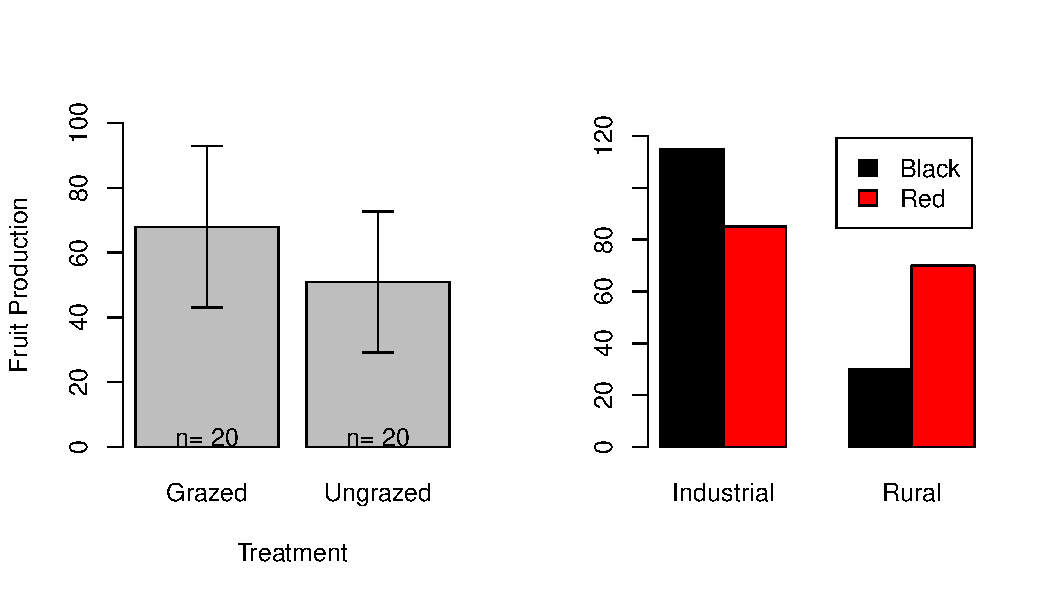
\includegraphics{Bio144_2017_week1-017}
\end{center}
}

\frame[containsverbatim]{\frametitle{Coplots}
Ideal zur Darstellung von Abh\"angigkeiten, wenn mehrere Variablen involviert sind. Eignet sich sehr gut bei kategoriellen Variablen. Beispiel: Quecksilber im Wallis.

\begin{center}
\setkeys{Gin}{width=0.7\textwidth}
\begin{Schunk}
\begin{Sinput}
> coplot(log(Hg_urin) ~  age | mother * migration ,d.hg,panel=panel.smooth)
\end{Sinput}
\end{Schunk}
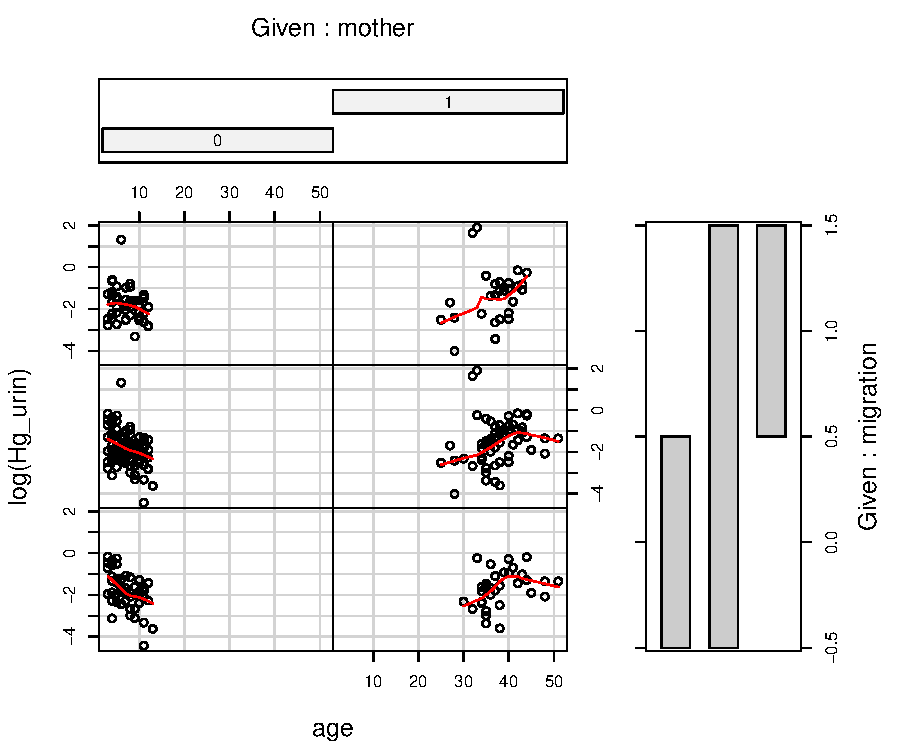
\includegraphics{Bio144_2017_week1-coplot}
\end{center}

}

\frame[containsverbatim]{\frametitle{}
Es gibt viele ``fancy'' Arten, Daten graphisch darzustellen ({\bf nice-to-know}):

\begin{itemize}
\item 3D-plots\\[1mm]
\item R\"aumliche Darstellungen (mit Geodaten)\\[1mm]
\item Interaktive Grafiken und Animationen\\[6mm]
\end{itemize}

Dazu gibt es etlich R Pakete. Interaktive Darstellungen k\"onnen beispielsweise mit Shiny Apps generiert werden (see census app).
%' <<>>=
%' library(shiny)
%' runApp("/home/steffi/Shiny/Tutorial/census-app")
%' @
}

\frame{\frametitle{N\"achste Woche: Einfache lineare Regression}

}



\frame{References:
\bibliographystyle{Chicago}
\bibliography{refs}
}




%\frame[containsverbatim]{\frametitle{Conditional density plots}
%Ideal, um Einfluss einer kontinuierlichen Variable auf einen bin\"aren Outcome (z.B. krank ja/nein) darzustellen
%\begin{center}
%<<echo=T>>=
%par(mfrow=c(1,1))
%fail <- factor(c(2, 2, 2, 2, 1, 1, 1, 1, 1, 1, 2, 1, 2, 1, 1, 1,1, 2, 1, 1, 1, 1, 1),
%               levels = 1:2, labels = c("no", "yes"))
%temperature <- c(53, 57, 58, 63, 66, 67, 67, 67, 68, 69, 70, 70,
%                 70, 70, 72, 73, 75, 75, 76, 76, 78, 79, 81)
%@
%\setkeys{Gin}{width=0.5\textwidth}
%<<cdplot,fig=T,echo=T,width=4,height=4>>=
%cdens <- cdplot(fail ~ temperature)
%@
%\end{center}
%}


\end{document}
